% ============================================================================
% CHƯƠNG 4: PARALLEL REDUCTION
% ============================================================================
\chapter{Parallel Reduction}
\label{chap:reduction}

\section{Giới thiệu về Reduction}

\subsection{Khái niệm}

\textbf{Reduction} (Rút gọn) là mẫu thuật toán cho phép rút gọn một tập hợp dữ liệu lớn thành một giá trị vô hướng (scalar) thông qua một phép toán kết hợp (associative operation).

Các phép toán reduction phổ biến:
\begin{itemize}
    \item \textbf{Sum}: $\sum_{i=0}^{n-1} a[i]$
    \item \textbf{Max}: $\max(a[0], a[1], ..., a[n-1])$
    \item \textbf{Min}: $\min(a[0], a[1], ..., a[n-1])$
    \item \textbf{Product}: $\prod_{i=0}^{n-1} a[i]$
\end{itemize}

\begin{figure}[H]
\centering
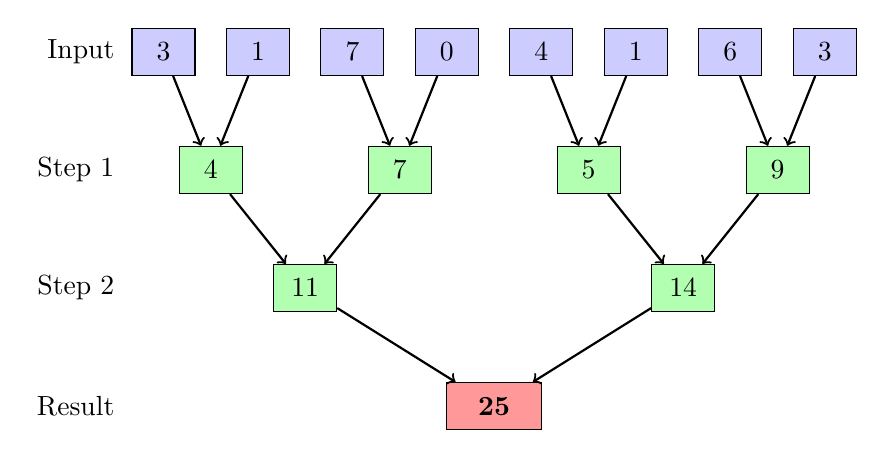
\begin{tikzpicture}[
    node distance=0.8cm,
    box/.style={draw, minimum width=0.8cm, minimum height=0.6cm, fill=blue!20},
    sumbox/.style={draw, minimum width=0.8cm, minimum height=0.6cm, fill=green!30},
    arrow/.style={->, thick}
]
    % Level 0: Input
    \foreach \i/\v in {0/3, 1/1, 2/7, 3/0, 4/4, 5/1, 6/6, 7/3} {
        \node[box] (a\i) at (\i*1.2, 0) {\v};
    }
    
    % Level 1
    \foreach \i/\v in {0/4, 1/7, 2/5, 3/9} {
        \node[sumbox] (b\i) at ({\i*2.4+0.6}, -1.5) {\v};
    }
    \draw[arrow] (a0) -- (b0);
    \draw[arrow] (a1) -- (b0);
    \draw[arrow] (a2) -- (b1);
    \draw[arrow] (a3) -- (b1);
    \draw[arrow] (a4) -- (b2);
    \draw[arrow] (a5) -- (b2);
    \draw[arrow] (a6) -- (b3);
    \draw[arrow] (a7) -- (b3);
    
    % Level 2
    \foreach \i/\v in {0/11, 1/14} {
        \node[sumbox] (c\i) at ({\i*4.8+1.8}, -3) {\v};
    }
    \draw[arrow] (b0) -- (c0);
    \draw[arrow] (b1) -- (c0);
    \draw[arrow] (b2) -- (c1);
    \draw[arrow] (b3) -- (c1);
    
    % Level 3: Result
    \node[sumbox, fill=red!40, minimum width=1.2cm] (d0) at (4.2, -4.5) {\textbf{25}};
    \draw[arrow] (c0) -- (d0);
    \draw[arrow] (c1) -- (d0);
    
    % Labels
    \node[left] at (-0.5, 0) {Input};
    \node[left] at (-0.5, -1.5) {Step 1};
    \node[left] at (-0.5, -3) {Step 2};
    \node[left] at (-0.5, -4.5) {Result};
    
\end{tikzpicture}
\caption{Cây Reduction cho phép tính Sum}
\label{fig:reduction_tree}
\end{figure}

\subsection{Serial Reduction}

Phiên bản tuần tự đơn giản:

\begin{lstlisting}[caption={Serial Reduction trên CPU}, label={lst:serial_reduction}]
// Ham reduction tong quat voi con tro ham
int reduce(const int *a, int n, int (*op)(int, int), int init) {
    int result = init;
    for (int i = 0; i < n; i++) {
        result = (*op)(result, a[i]);
    }
    return result;
}

// Cac phep toan
int add(int a, int b) { return a + b; }
int max_op(int a, int b) { return (a > b) ? a : b; }
int product(int a, int b) { return a * b; }

// Su dung
int sum = reduce(arr, n, add, 0);
int maximum = reduce(arr, n, max_op, arr[0]);
int prod = reduce(arr, n, product, 1);
\end{lstlisting}

\textbf{Độ phức tạp:} $O(n)$ - mỗi phần tử được xử lý một lần.

\section{Parallel Reduction - Phiên bản cơ bản}

\subsection{Ý tưởng}

Chia dữ liệu thành các block, mỗi block tính partial sum, sau đó cộng các partial sums lại.

\begin{figure}[H]
\centering
\begin{tikzpicture}[scale=0.75]
    % Data array
    \foreach \i in {0,...,15} {
        \draw[fill=blue!20] (\i*0.7, 4) rectangle ++(0.6, 0.5);
        \node[font=\tiny] at ({\i*0.7+0.3}, 4.25) {\i};
    }
    
    % Block boundaries
    \draw[very thick, red] (0, 3.9) rectangle (2.8, 4.6);
    \draw[very thick, green!50!black] (2.8, 3.9) rectangle (5.6, 4.6);
    \draw[very thick, blue] (5.6, 3.9) rectangle (8.4, 4.6);
    \draw[very thick, orange] (8.4, 3.9) rectangle (11.2, 4.6);
    
    % Partial sums
    \node[draw, fill=red!30, minimum width=1.5cm] (p0) at (1.4, 2.5) {P0};
    \node[draw, fill=green!30, minimum width=1.5cm] (p1) at (4.2, 2.5) {P1};
    \node[draw, fill=blue!30, minimum width=1.5cm] (p2) at (7, 2.5) {P2};
    \node[draw, fill=orange!30, minimum width=1.5cm] (p3) at (9.8, 2.5) {P3};
    
    % Arrows to partial sums
    \draw[->] (1.4, 3.9) -- (p0);
    \draw[->] (4.2, 3.9) -- (p1);
    \draw[->] (7, 3.9) -- (p2);
    \draw[->] (9.8, 3.9) -- (p3);
    
    % Final sum on CPU
    \node[draw, fill=purple!30, minimum width=2cm] (total) at (5.6, 0.8) {Total Sum};
    \draw[->] (p0) -- (total);
    \draw[->] (p1) -- (total);
    \draw[->] (p2) -- (total);
    \draw[->] (p3) -- (total);
    
    \node[font=\footnotesize] at (5.6, 0) {(Cộng trên CPU)};
    
\end{tikzpicture}
\caption{Parallel Reduction: Mỗi block tính partial sum}
\label{fig:parallel_reduction_blocks}
\end{figure}

\subsection{Thuật toán reduceNeighbors (Phiên bản 1)}

Cặp các phần tử liền kề trong mỗi bước:

\begin{lstlisting}[caption={Parallel Reduction - reduceNeighbors}, label={lst:reduce_neighbors}]
__global__ void reduceNeighbors(int *diData, int *doData, int n) {
    int stride;
    int idx = threadIdx.x;
    int *iData = diData + blockIdx.x * blockDim.x;
    
    // Reduction loop
    for (stride = 1; stride < blockDim.x; stride *= 2) {
        // Chi threads co idx % (2*stride) == 0 tham gia
        if ((idx % (2 * stride)) == 0) {
            iData[idx] += iData[idx + stride];
        }
        __syncthreads();  // Dong bo sau moi buoc
    }
    
    // Thread 0 ghi ket qua
    if (idx == 0) {
        doData[blockIdx.x] = iData[0];
    }
}
\end{lstlisting}

\begin{figure}[H]
\centering
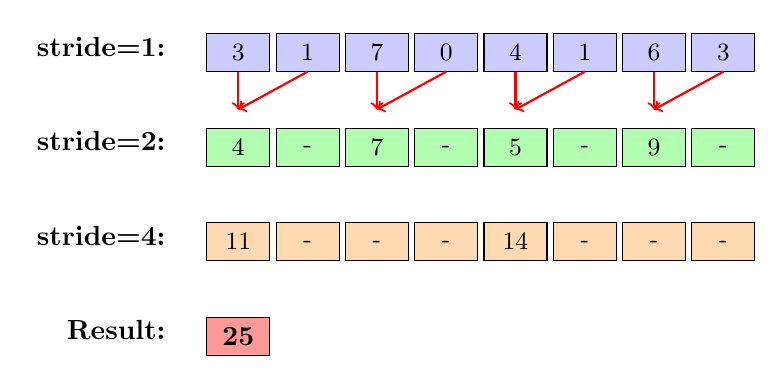
\begin{tikzpicture}[scale=0.8]
    % Step 0
    \node[left, font=\bfseries] at (-0.5, 3) {stride=1:};
    \foreach \i/\v in {0/3, 1/1, 2/7, 3/0, 4/4, 5/1, 6/6, 7/3} {
        \draw[fill=blue!20] (\i*1.1, 2.6) rectangle ++(1, 0.6);
        \node[font=\small] at ({\i*1.1+0.5}, 2.9) {\v};
    }
    \foreach \i in {0,2,4,6} {
        \draw[->, thick, red] ({\i*1.1+0.5}, 2.6) -- ({\i*1.1+0.5}, 2);
        \draw[->, thick, red] ({(\i+1)*1.1+0.5}, 2.6) -- ({\i*1.1+0.5}, 2);
    }
    
    % Step 1
    \node[left, font=\bfseries] at (-0.5, 1.5) {stride=2:};
    \foreach \i/\v in {0/4, 1/-, 2/7, 3/-, 4/5, 5/-, 6/9, 7/-} {
        \ifx\v-
            \draw[fill=gray!20] (\i*1.1, 1.1) rectangle ++(1, 0.6);
        \else
            \draw[fill=green!30] (\i*1.1, 1.1) rectangle ++(1, 0.6);
            \node[font=\small] at ({\i*1.1+0.5}, 1.4) {\v};
        \fi
    }
    
    % Step 2
    \node[left, font=\bfseries] at (-0.5, 0) {stride=4:};
    \foreach \i/\v in {0/11, 1/-, 2/-, 3/-, 4/14, 5/-, 6/-, 7/-} {
        \ifx\v-
            \draw[fill=gray!20] (\i*1.1, -0.4) rectangle ++(1, 0.6);
        \else
            \draw[fill=orange!30] (\i*1.1, -0.4) rectangle ++(1, 0.6);
            \node[font=\small] at ({\i*1.1+0.5}, -0.1) {\v};
        \fi
    }
    
    % Final
    \node[left, font=\bfseries] at (-0.5, -1.5) {Result:};
    \draw[fill=red!40] (0, -1.9) rectangle ++(1, 0.6);
    \node[font=\bfseries] at (0.5, -1.6) {25};
    
\end{tikzpicture}
\caption{Quá trình thực thi reduceNeighbors}
\label{fig:reduce_neighbors_steps}
\end{figure}

\textbf{Vấn đề:} Thuật toán này gây ra \textbf{Warp Divergence} nghiêm trọng:
\begin{itemize}
    \item Stride = 1: Chỉ 50\% threads hoạt động
    \item Stride = 2: Chỉ 25\% threads hoạt động
    \item Stride = 4: Chỉ 12.5\% threads hoạt động
    \item ...
\end{itemize}

\section{Parallel Reduction - Phiên bản tối ưu}

\subsection{reduceNeighbors2 - Giảm Warp Divergence}

Sắp xếp lại để các threads liên tiếp cùng hoạt động:

\begin{lstlisting}[caption={Parallel Reduction - reduceNeighbors2}, label={lst:reduce_neighbors2}]
__global__ void reduceNeighbors2(int *diData, int *doData, int n) {
    int stride;
    int tid = threadIdx.x;
    int *iData = diData + blockIdx.x * blockDim.x;
    
    for (stride = 1; stride < blockDim.x; stride *= 2) {
        // Tinh index moi de cac threads lien tiep hoat dong
        int index = 2 * stride * tid;
        
        if (index < blockDim.x) {
            iData[index] += iData[index + stride];
        }
        __syncthreads();
    }
    
    if (tid == 0) {
        doData[blockIdx.x] = iData[0];
    }
}
\end{lstlisting}

\textbf{Cải thiện:} Các threads 0, 1, 2, ... $\lfloor\frac{blockDim}{2 \times stride}\rfloor$ cùng hoạt động trong mỗi bước, giảm warp divergence.

\subsection{reduceInterLeaves - Interleaved Pair}

Cặp các phần tử cách nhau stride, bắt đầu từ stride = blockDim/2:

\begin{lstlisting}[caption={Parallel Reduction - Interleaved Pair}, label={lst:reduce_interleaved}]
__global__ void reduceInterLeaves(int *diData, int *doData, int n) {
    int stride;
    int tid = threadIdx.x;
    int *iData = diData + blockIdx.x * blockDim.x;
    
    // Bat dau tu stride = blockDim/2, giam dan
    for (stride = blockDim.x / 2; stride > 0; stride >>= 1) {
        if (tid < stride) {
            iData[tid] += iData[tid + stride];
        }
        __syncthreads();
    }
    
    if (tid == 0) {
        doData[blockIdx.x] = iData[0];
    }
}
\end{lstlisting}

\begin{figure}[H]
\centering
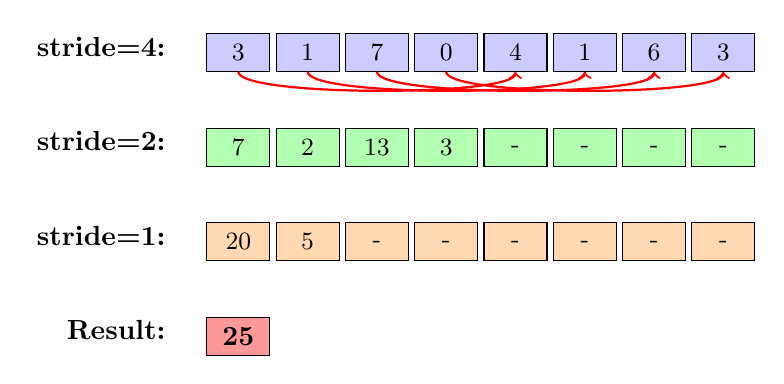
\begin{tikzpicture}[scale=0.8]
    % Initial
    \node[left, font=\bfseries] at (-0.5, 4) {stride=4:};
    \foreach \i/\v in {0/3, 1/1, 2/7, 3/0, 4/4, 5/1, 6/6, 7/3} {
        \draw[fill=blue!20] (\i*1.1, 3.6) rectangle ++(1, 0.6);
        \node[font=\small] at ({\i*1.1+0.5}, 3.9) {\v};
    }
    
    % Arrows for stride=4
    \foreach \i in {0,1,2,3} {
        \draw[->, thick, red] ({\i*1.1+0.5}, 3.6) .. controls ({\i*1.1+0.5}, 3.2) and ({(\i+4)*1.1+0.5}, 3.2) .. ({(\i+4)*1.1+0.5}, 3.6);
    }
    
    % Step 1: stride=4 result
    \node[left, font=\bfseries] at (-0.5, 2.5) {stride=2:};
    \foreach \i/\v in {0/7, 1/2, 2/13, 3/3, 4/-, 5/-, 6/-, 7/-} {
        \ifx\v-
            \draw[fill=gray!20] (\i*1.1, 2.1) rectangle ++(1, 0.6);
        \else
            \draw[fill=green!30] (\i*1.1, 2.1) rectangle ++(1, 0.6);
            \node[font=\small] at ({\i*1.1+0.5}, 2.4) {\v};
        \fi
    }
    
    % Step 2: stride=2 result
    \node[left, font=\bfseries] at (-0.5, 1) {stride=1:};
    \foreach \i/\v in {0/20, 1/5, 2/-, 3/-, 4/-, 5/-, 6/-, 7/-} {
        \ifx\v-
            \draw[fill=gray!20] (\i*1.1, 0.6) rectangle ++(1, 0.6);
        \else
            \draw[fill=orange!30] (\i*1.1, 0.6) rectangle ++(1, 0.6);
            \node[font=\small] at ({\i*1.1+0.5}, 0.9) {\v};
        \fi
    }
    
    % Final
    \node[left, font=\bfseries] at (-0.5, -0.5) {Result:};
    \draw[fill=red!40] (0, -0.9) rectangle ++(1, 0.6);
    \node[font=\bfseries] at (0.5, -0.6) {25};
    
\end{tikzpicture}
\caption{Quá trình thực thi reduceInterLeaves}
\label{fig:reduce_interleaved_steps}
\end{figure}

\textbf{Ưu điểm của Interleaved:}
\begin{itemize}
    \item Memory coalescing tốt hơn trong bước đầu
    \item Giảm bank conflicts trong shared memory
    \item Các threads liên tiếp truy cập bộ nhớ liên tiếp
\end{itemize}

\section{So sánh hiệu năng}

\subsection{Benchmark với các kích thước khác nhau}

\begin{lstlisting}[caption={Hàm benchmark reduction}, label={lst:benchmark_reduction}]
float runReduction(void (*kernel)(int*, int*, int), 
                   int *dA, int *dB, int *hb,
                   int n, int gridSize, int blockSize, 
                   const char *name) {
    cudaEvent_t start, stop;
    cudaEventCreate(&start);
    cudaEventCreate(&stop);
    
    dim3 block(blockSize, 1);
    dim3 grid(gridSize, 1);
    
    cudaEventRecord(start);
    kernel<<<grid, block>>>(dA, dB, n);
    cudaDeviceSynchronize();
    cudaEventRecord(stop);
    cudaEventSynchronize(stop);
    
    float milliseconds = 0;
    cudaEventElapsedTime(&milliseconds, start, stop);
    
    // Tinh tong tu partial sums
    cudaMemcpy(hb, dB, gridSize * sizeof(int), cudaMemcpyDeviceToHost);
    int sum = 0;
    for (int i = 0; i < gridSize; i++) sum += hb[i];
    
    printf("%s - Sum: %d, Time: %.4f ms\n", name, sum, milliseconds);
    
    return milliseconds;
}
\end{lstlisting}

\begin{table}[H]
\centering
\caption{So sánh hiệu năng 3 thuật toán Parallel Reduction}
\label{tab:reduction_comparison}
\begin{tabular}{@{}lcccc@{}}
\toprule
\textbf{Input Size} & \textbf{reduceNeighbors} & \textbf{reduceNeighbors2} & \textbf{reduceInterLeaves} & \textbf{Best Speedup} \\
\midrule
$2^{16}$ (65K) & 0.0312 ms & 0.0245 ms & 0.0198 ms & 1.58x \\
$2^{18}$ (262K) & 0.0892 ms & 0.0678 ms & 0.0512 ms & 1.74x \\
$2^{20}$ (1M) & 0.3245 ms & 0.2456 ms & 0.1823 ms & 1.78x \\
$2^{22}$ (4M) & 1.2134 ms & 0.9234 ms & 0.6823 ms & 1.78x \\
$2^{24}$ (16M) & 4.7823 ms & 3.6234 ms & 2.6789 ms & 1.79x \\
\bottomrule
\end{tabular}
\end{table}

\begin{figure}[H]
\centering
\begin{tikzpicture}
\begin{axis}[
    width=13cm,
    height=8cm,
    xlabel={Input Size ($\log_2 n$)},
    ylabel={Execution Time (ms)},
    xmin=15, xmax=25,
    ymin=0, ymax=5.5,
    legend pos=north west,
    grid=both,
    grid style={gray!30},
    title={So sánh hiệu năng 3 thuật toán Parallel Reduction}
]
\addplot[thick, mark=square*, red] coordinates {
    (16, 0.0312)
    (18, 0.0892)
    (20, 0.3245)
    (22, 1.2134)
    (24, 4.7823)
};
\addlegendentry{reduceNeighbors}

\addplot[thick, mark=triangle*, blue] coordinates {
    (16, 0.0245)
    (18, 0.0678)
    (20, 0.2456)
    (22, 0.9234)
    (24, 3.6234)
};
\addlegendentry{reduceNeighbors2}

\addplot[thick, mark=o, green!50!black] coordinates {
    (16, 0.0198)
    (18, 0.0512)
    (20, 0.1823)
    (22, 0.6823)
    (24, 2.6789)
};
\addlegendentry{reduceInterLeaves}
\end{axis}
\end{tikzpicture}
\caption{Biểu đồ so sánh thời gian thực thi}
\label{fig:reduction_perf_chart}
\end{figure}

\subsection{Phân tích}

\begin{table}[H]
\centering
\caption{Phân tích ưu nhược điểm các thuật toán}
\label{tab:reduction_analysis}
\begin{tabular}{@{}lp{4cm}p{4cm}p{4cm}@{}}
\toprule
\textbf{Thuật toán} & \textbf{Ưu điểm} & \textbf{Nhược điểm} & \textbf{Warp Divergence} \\
\midrule
reduceNeighbors & Đơn giản, dễ hiểu & Divergence cao, memory access pattern kém & Cao \\
\midrule
reduceNeighbors2 & Giảm divergence đáng kể & Vẫn còn bank conflicts & Trung bình \\
\midrule
reduceInterLeaves & Memory coalescing tốt, ít bank conflicts & Phức tạp hơn một chút & Thấp \\
\bottomrule
\end{tabular}
\end{table}

\section{Bài tập mở rộng: Float Reduction}

\begin{lstlisting}[caption={Parallel Reduction với kiểu Float}, label={lst:float_reduction}]
__global__ void reduceInterLeavesFloat(float *diData, float *doData, int n) {
    int stride;
    int tid = threadIdx.x;
    float *iData = diData + blockIdx.x * blockDim.x;
    
    for (stride = blockDim.x / 2; stride > 0; stride >>= 1) {
        if (tid < stride) {
            iData[tid] += iData[tid + stride];
        }
        __syncthreads();
    }
    
    if (tid == 0) {
        doData[blockIdx.x] = iData[0];
    }
}
\end{lstlisting}

\textbf{Lưu ý với Float:}
\begin{itemize}
    \item Kết quả có thể khác nhau do thứ tự cộng (floating-point không associative hoàn toàn)
    \item Sai số tích lũy có thể xảy ra với dữ liệu lớn
    \item Sử dụng Kahan summation nếu cần độ chính xác cao
\end{itemize}

\section{Kết luận chương}

Chương này đã trình bày chi tiết về Parallel Reduction:

\begin{itemize}
    \item \textbf{Khái niệm}: Rút gọn mảng thành scalar qua phép toán kết hợp
    \item \textbf{Ba thuật toán}: reduceNeighbors, reduceNeighbors2, reduceInterLeaves
    \item \textbf{Tối ưu hóa}: 
        \begin{itemize}
            \item Giảm warp divergence
            \item Cải thiện memory coalescing
            \item Tránh bank conflicts
        \end{itemize}
    \item \textbf{Hiệu năng}: reduceInterLeaves nhanh gấp ~1.8x so với reduceNeighbors
\end{itemize}

Reduction là pattern quan trọng, được sử dụng trong nhiều thuật toán phức tạp hơn như Dot Product (Chương 5) và Sorting (Chương 6-7).
